% Universidade Aberta
% Template TeX para relatório de trabalhos
% 2024
%
%
% Dados para a capa
\newcommand{\Titulo}{Plataforma de Questionários\\Programação Web Avançada 2024}
\newcommand{\Ano}{2025}
\newcommand{\Autor}{Hugo Gonçalves}
%
%
\documentclass[12pt,a4paper,final]{article}
\usepackage[stretch=10]{microtype}
\usepackage{csquotes}
\usepackage[portuguese]{babel}
\usepackage{polyglossia}
\setdefaultlanguage{portuguese}
\usepackage{graphicx}
\graphicspath{ {./images/} }
\usepackage[a4paper,top=3cm,bottom=3cm,left=3.5cm,right=2cm]{geometry}
\usepackage{booktabs}
\usepackage{newtxtext}
\usepackage{newtxmath}
\usepackage{pgf-umlsd}
\usepackage[pdfauthor=\Autor,
    pdftitle=\Titulo,
    colorlinks=true,
    linkcolor=black,
    citecolor=black,
    bookmarksopen=true]{hyperref}
\hypersetup{colorlinks, citecolor=black, urlcolor=black}
\usepackage{bookmark}
\usepackage{float}
\usepackage[style=apa, backend=biber, sortcites, url=true]{biblatex}
\addbibresource{ref.bib}
\renewcommand{\baselinestretch}{1.5}
\begin{document}
    \title{\Titulo}
    \author{\Autor}
    \date{\Ano}
    \pagenumbering{gobble}
    \begin{titlepage}
        \begin{center}
            \vspace*{4cm}

            \textbf{\large UNIVERSIDADE ABERTA}

            \textbf{\large UNIVERSIDADE DE TRÁS-OS-MONTES E ALTO DOURO}

            \vspace{1cm}

            \begin{minipage}{0.4\textwidth}
                \centering
                
\includegraphics[width=0.8\textwidth]{uab}
            \end{minipage}
            \begin{minipage}{0.4\textwidth}
                \centering
                
\includegraphics[width=0.8\textwidth]{utad}
            \end{minipage}

            \vspace{1.5cm}

            \textbf{\large \Titulo}

            \vspace{1.5cm}

            \textbf{\large \Autor}

            \vspace{2cm}

            \textbf{\large Mestrado em Engenharia Informática e Tecnologia Web}
            \vfill
            \textbf{\Ano}
        \end{center}
    \end{titlepage}
    \renewcommand{\contentsname}{Índice}
    \cleardoublepage
    \pagenumbering{roman}
    \tableofcontents
    \newpage
    \listoffigures
    \newpage
    \cleardoublepage
    \pagenumbering{arabic}


    \section{Introdução}\label{sec:introducao}
    No âmbito do projeto final da unidade curricular de Programação Web Avançada, projetou-se e desenvolveu-se uma plataforma de questionários que permite que formadores criem questionários com perguntas de escolha múltipla.
    A plataforma apenas permite o registo automático de utilizadores do tipo estudante, e, este tipo de utilizador é apresentado com uma página que lista todos os questionários que tem por responder.
    Ao responder a um questionário, o mesmo desaparece da página inicial.
    Ao utilizador do tipo formador, é apresentado, na página inicial, uma listagem de todos os seus questionários, oferecendo uma ligação para um resumo de cada um, onde é apresentada uma lista de utilizadores que responderam ao questionário bem como o número de respostas erradas e corretas.
    A plataforma está dividida entre \textit{Frontend}, \textit{Backend} e base de dados NoSQL\@ e as várias etapas do seu desenvolvimento podem ser acompanhadas no repositório disponível em \href{https://github.com/2100562/PWA-ProjetoFinal}{github.com/2100562/PWA-ProjetoFinal}.


    \section{Prototipagem}\label{sec:prototipagem}
    Para a prototipagem, utilizando o conceito \textit{Mobile-first}, começou-se por desenhar os \textit{wireframes} de cada página para dispositivos móveis, passando, depois, para o desenho dos mesmos para dispositivos \textit{Desktop}.
    Após os \textit{wireframes} estarem completos, passou-se ao desenvolvimento dos \textit{mockups} sem funcionalidade de negócio implementada, mas interativos.
    No interesse do tempo, os \textit{mockups} foram desenvolvidos já recorrendo a Vue.js.

    \subsection{Páginas do Formador}\label{subsec:paginas-do-formador}
    Para o utilizador do tipo formador, foram consideradas três páginas com funcionalidades específicas.

    \subsubsection{Página Inicial}
    A página inicial apresenta uma lista de questionários previamente criados pelo utilizador, oferecendo uma ligação para aceder a uma página de detalhe do questionário.

    \begin{figure}[H]
        \centering
        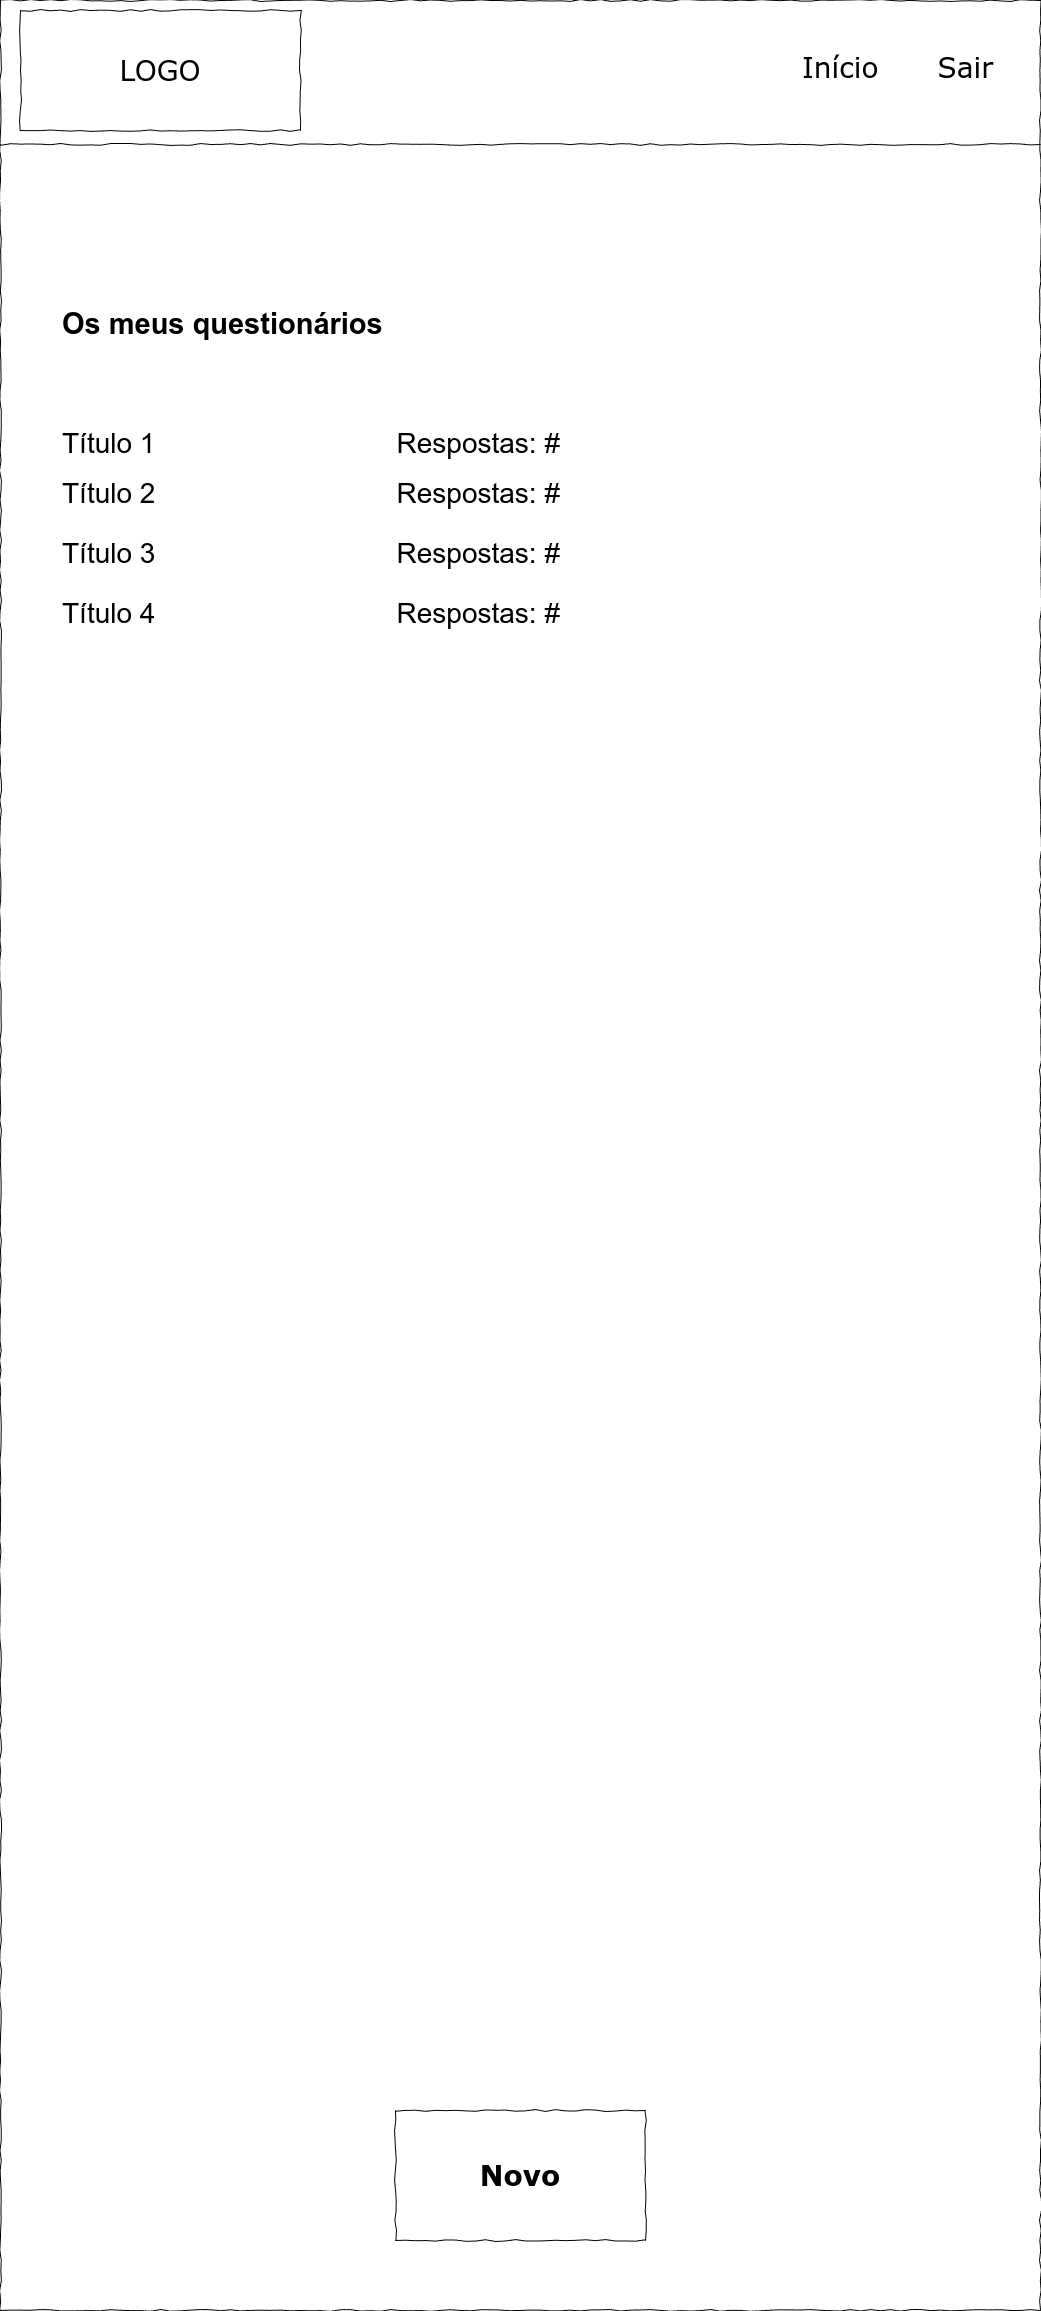
\includegraphics[width=\textwidth,height=0.9\textheight,keepaspectratio]{wireframes/questionarios.wireframes-formador-geral-mobile.drawio}
        \caption{\textit{Wireframe Mobile} - Página Inicial Formador}
        \label{fig:wm-pif}
    \end{figure}

    \begin{figure}[H]
        \centering
        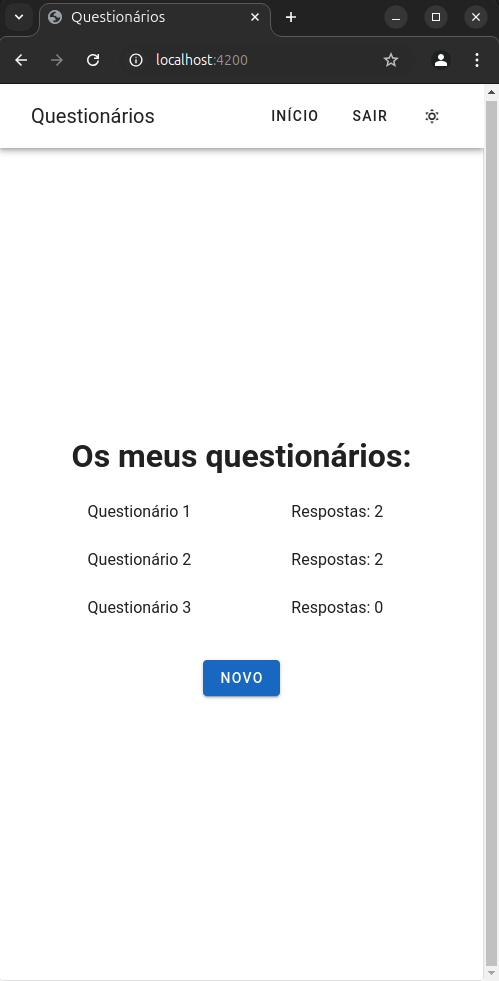
\includegraphics[width=\textwidth,height=0.9\textheight,keepaspectratio]{mockups/questionarios.wireframes-formador-geral-mobile}
        \caption{\textit{Mockup Mobile} - Página Inicial Formador}
        \label{fig:mm-pif}
    \end{figure}

    \begin{figure}[H]
        \centering
        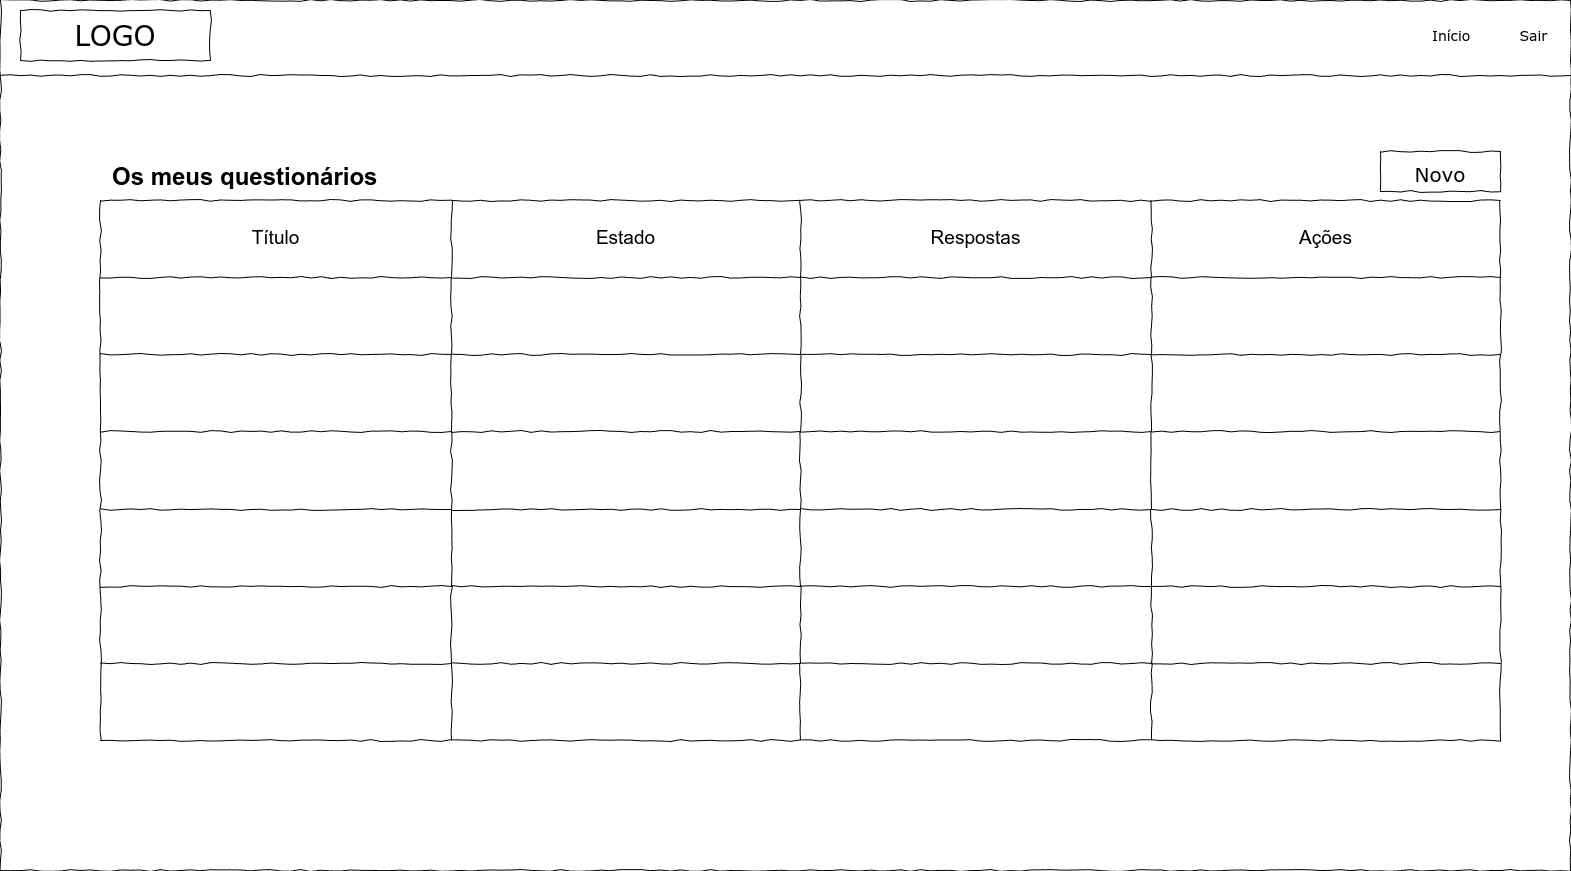
\includegraphics[width=\textwidth,height=0.9\textheight,keepaspectratio]{wireframes/questionarios.wireframes-formador-geral-desktop.drawio}
        \caption{\textit{Wireframe Desktop} - Página Inicial Formador}
        \label{fig:wd-pif}
    \end{figure}

    \begin{figure}[H]
        \centering
        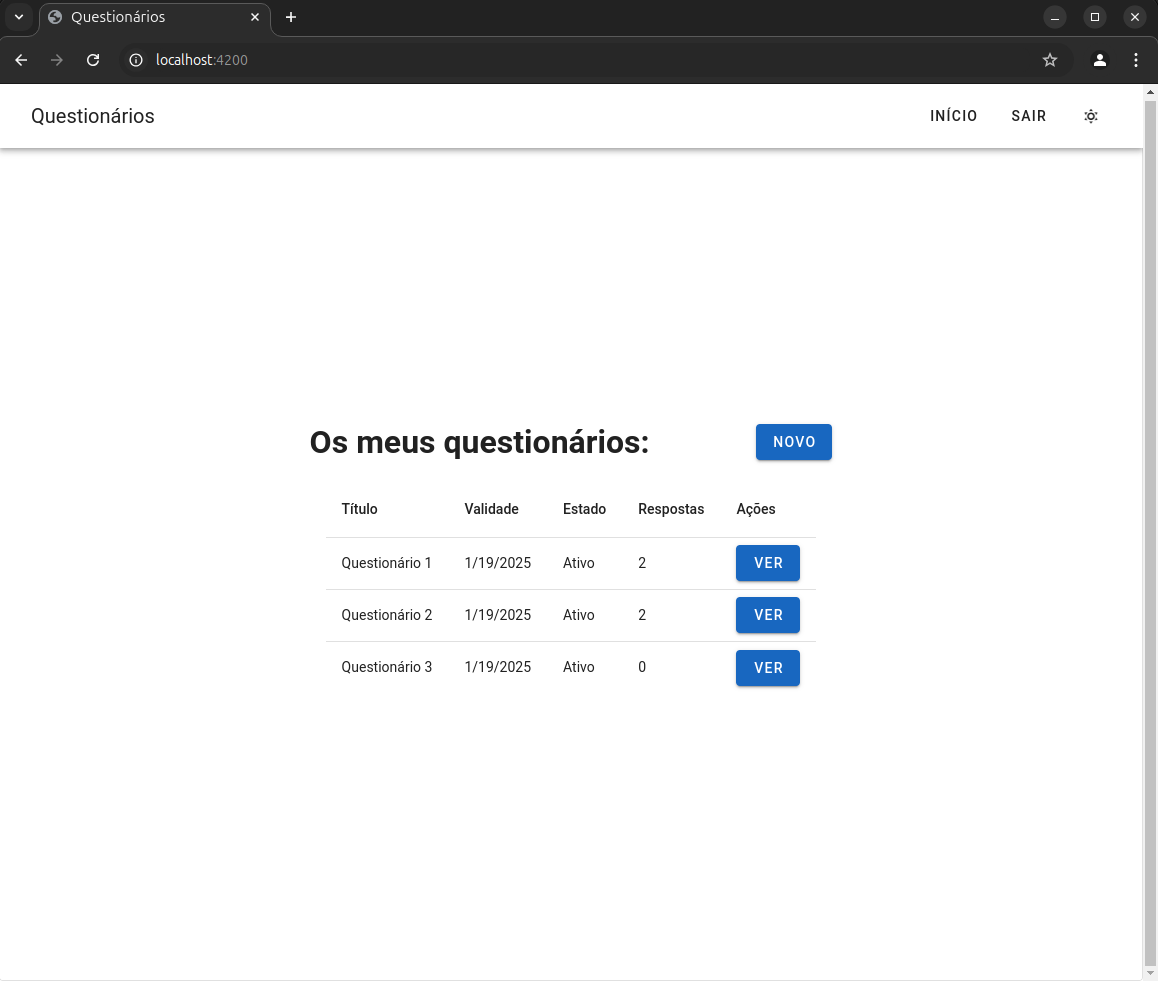
\includegraphics[width=\textwidth,height=0.9\textheight,keepaspectratio]{mockups/questionarios.wireframes-formador-geral-desktop}
        \caption{\textit{Mockup Desktop} - Página Inicial Formador}
        \label{fig:md-pif}
    \end{figure}

    \subsubsection{Página Questionário}
    Na página de questionário é apresentado o detalhe do questionário, listando os utilizadores que responderam ao questionário com a contagem de respostas corretas e erradas.

    \begin{figure}[H]
        \centering
        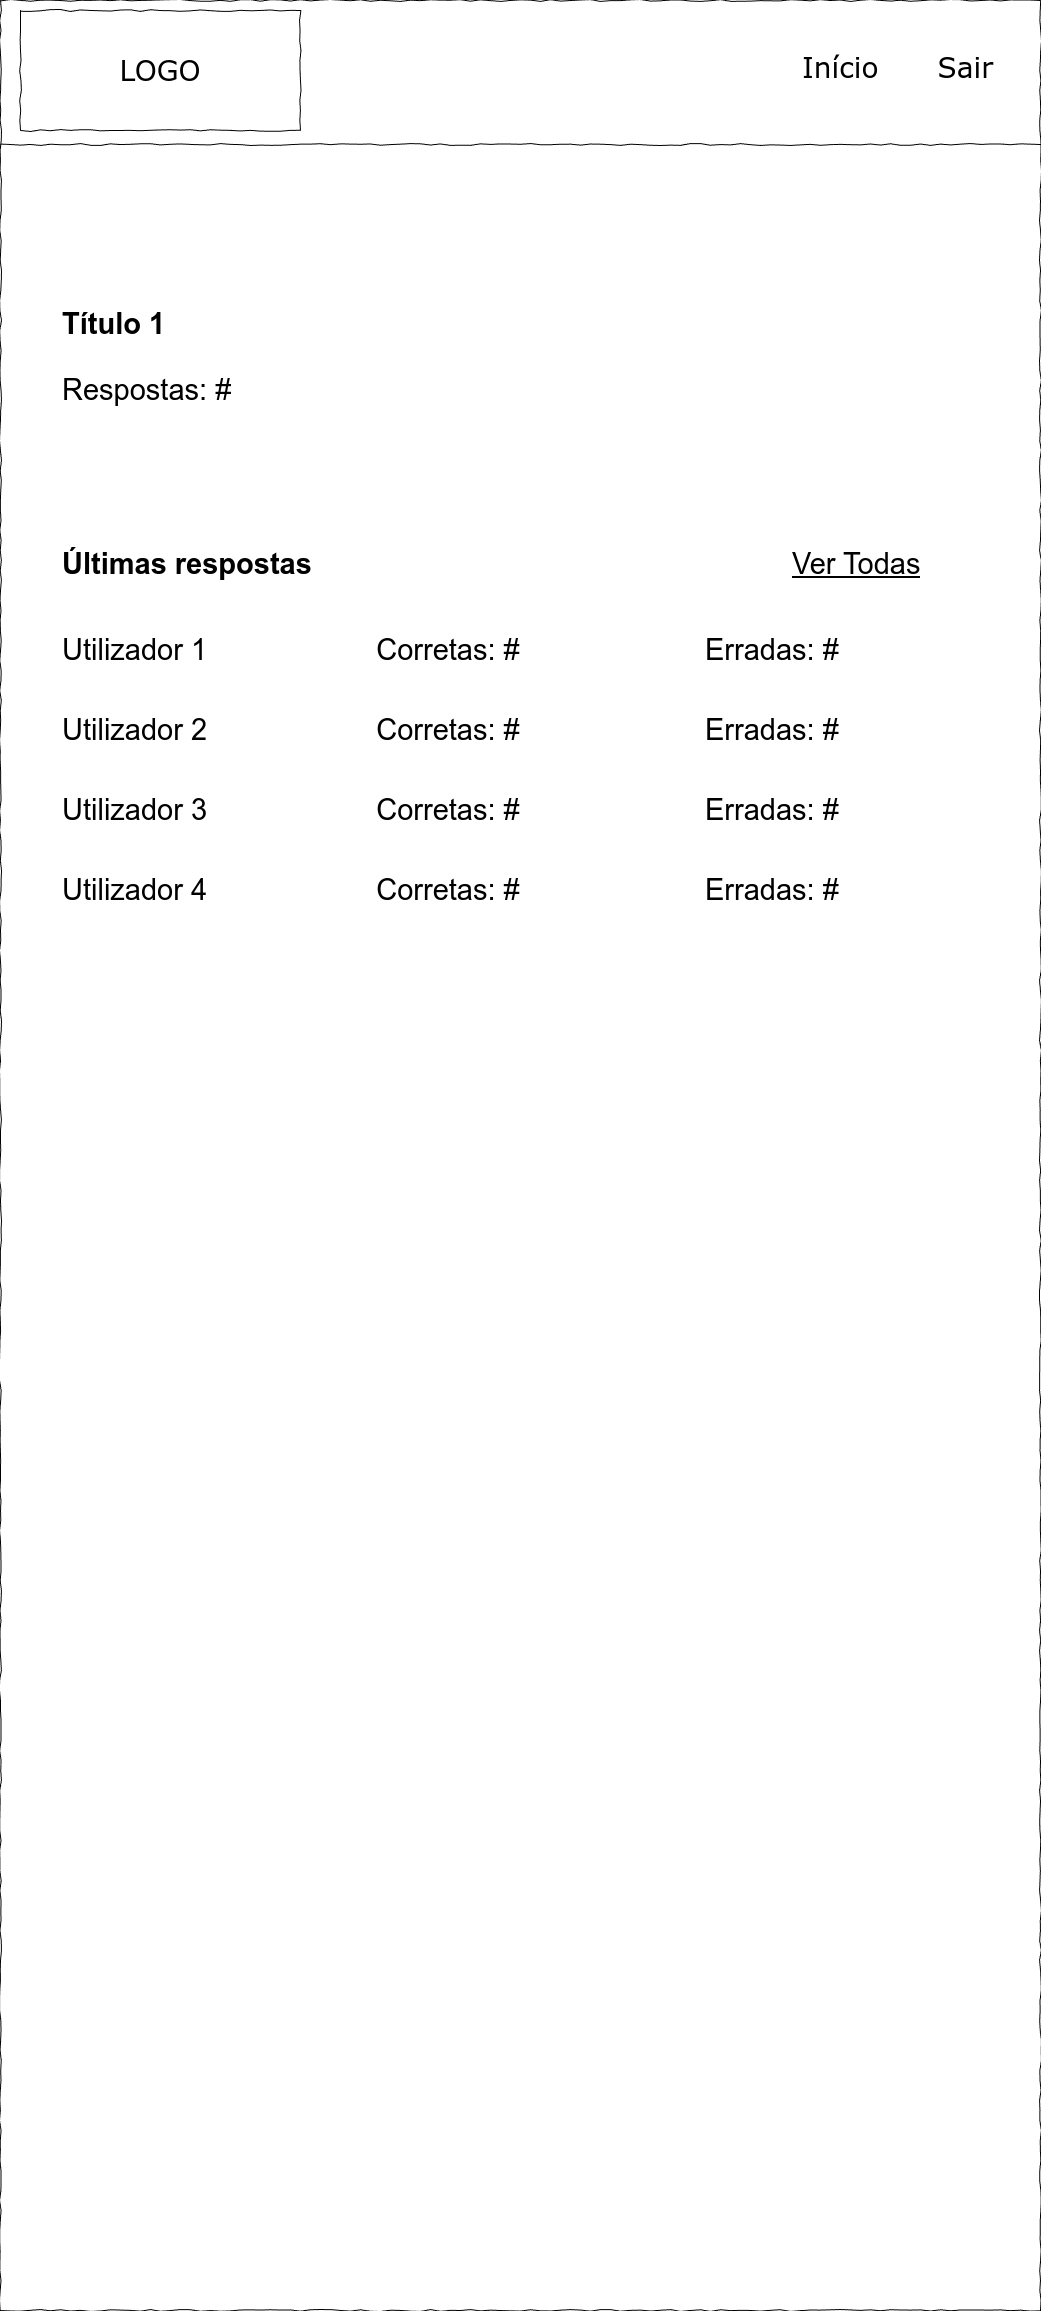
\includegraphics[width=\textwidth,height=0.9\textheight,keepaspectratio]{wireframes/questionarios.wireframes-formador-questionario-mobile.drawio}
        \caption{\textit{Wireframe Mobile} - Página Questionário Formador}
        \label{fig:wm-pqf}
    \end{figure}

    \begin{figure}[H]
        \centering
        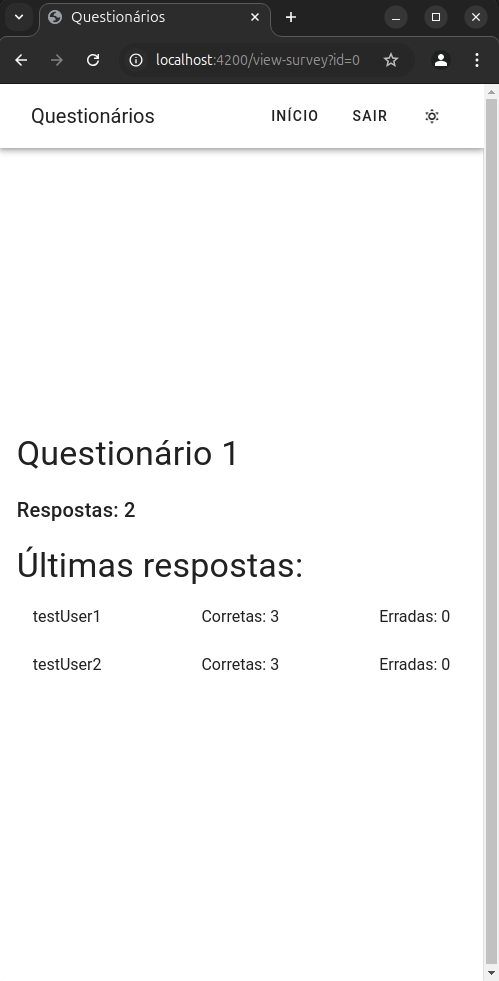
\includegraphics[width=\textwidth,height=0.9\textheight,keepaspectratio]{mockups/questionarios.wireframes-formador-questionario-mobile}
        \caption{\textit{Mockup Mobile} - Página Questionário Formador}
        \label{fig:mm-pqf}
    \end{figure}

    \begin{figure}[H]
        \centering
        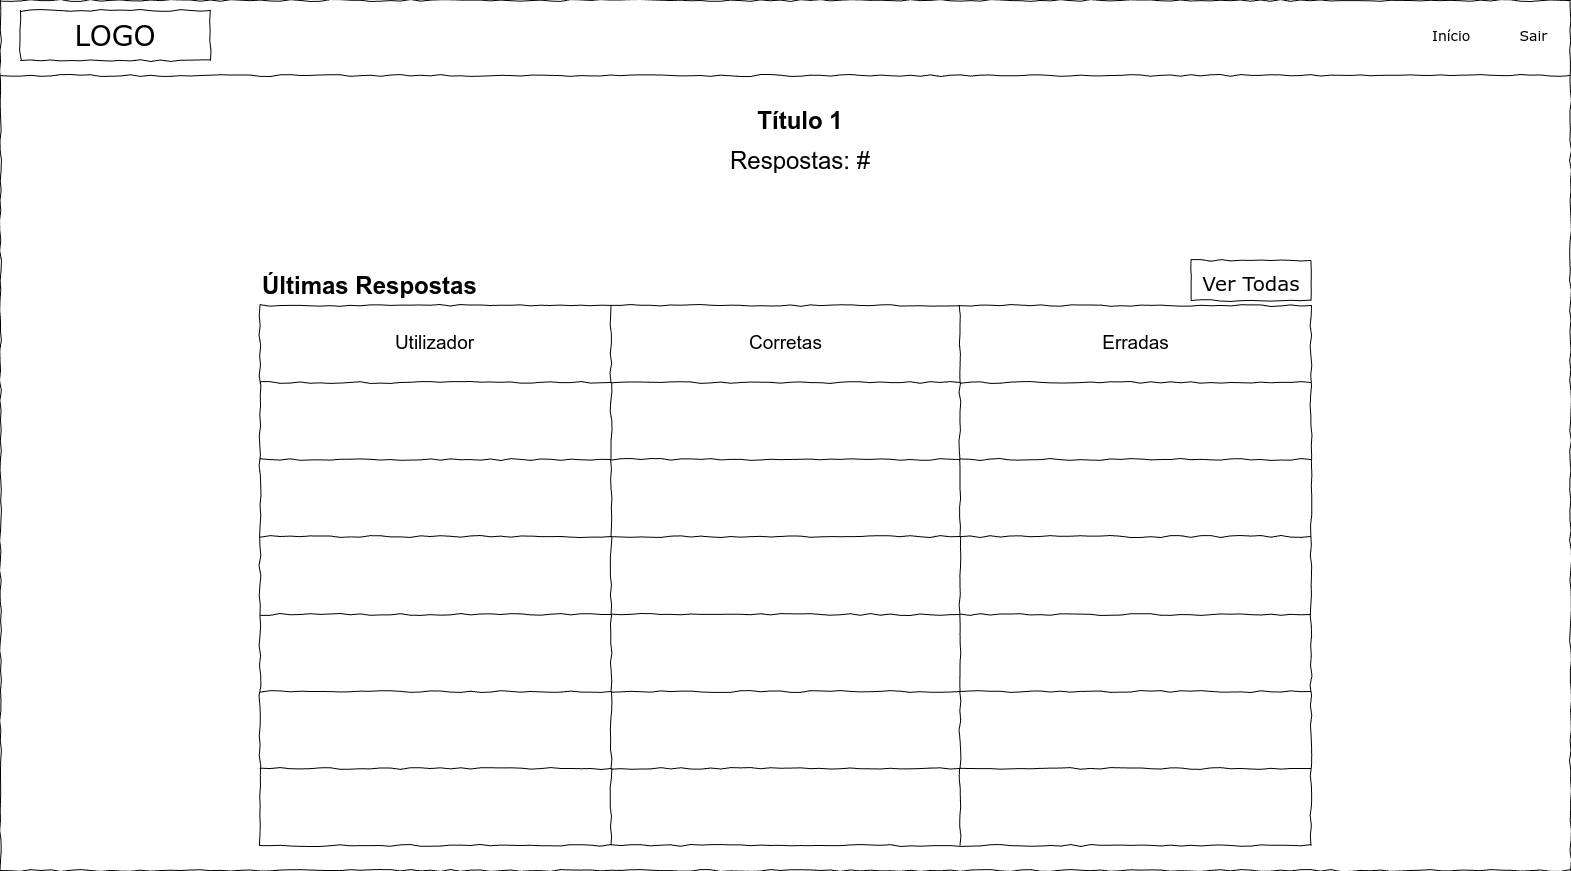
\includegraphics[width=\textwidth,height=0.9\textheight,keepaspectratio]{wireframes/questionarios.wireframes-formador-questionario-desktop.drawio}
        \caption{\textit{Wireframe Desktop} - Página Questionário Formador}
        \label{fig:wd-pqf}
    \end{figure}

    \begin{figure}[H]
        \centering
        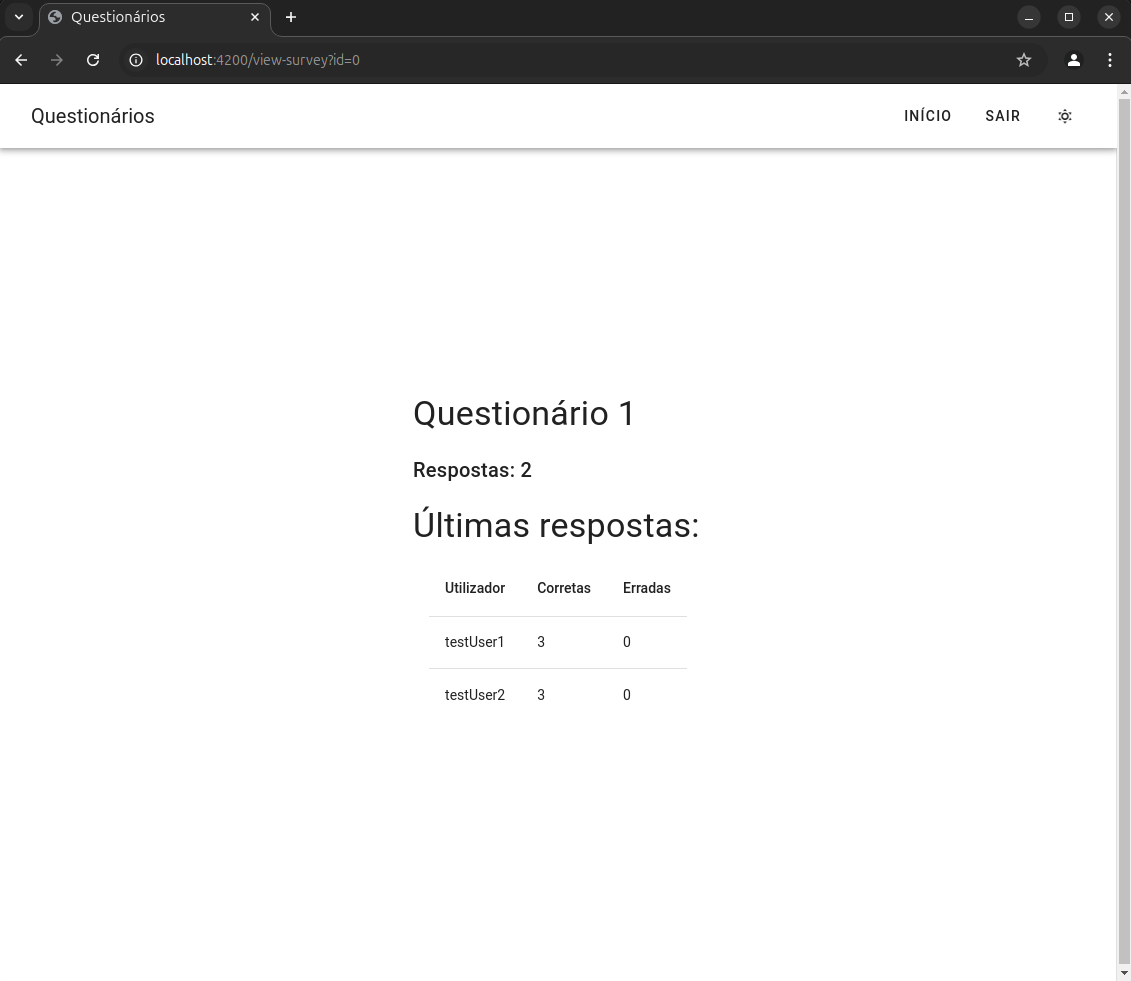
\includegraphics[width=\textwidth,height=0.9\textheight,keepaspectratio]{mockups/questionarios.wireframes-formador-questionario-desktop}
        \caption{\textit{Mockup Desktop} - Página Questionário Formador}
        \label{fig:md-pqf}
    \end{figure}

    \subsubsection{Página Novo Questionário}
    Na página de criação de questionários, é apresentado um formulário onde o formador pode preencher o título bem como a data de validade do questionário.
    Um questionário deverá ter pelo menos uma pergunta, e, dinamicamente o formador pode adicionar mais.

    \begin{figure}[H]
        \centering
        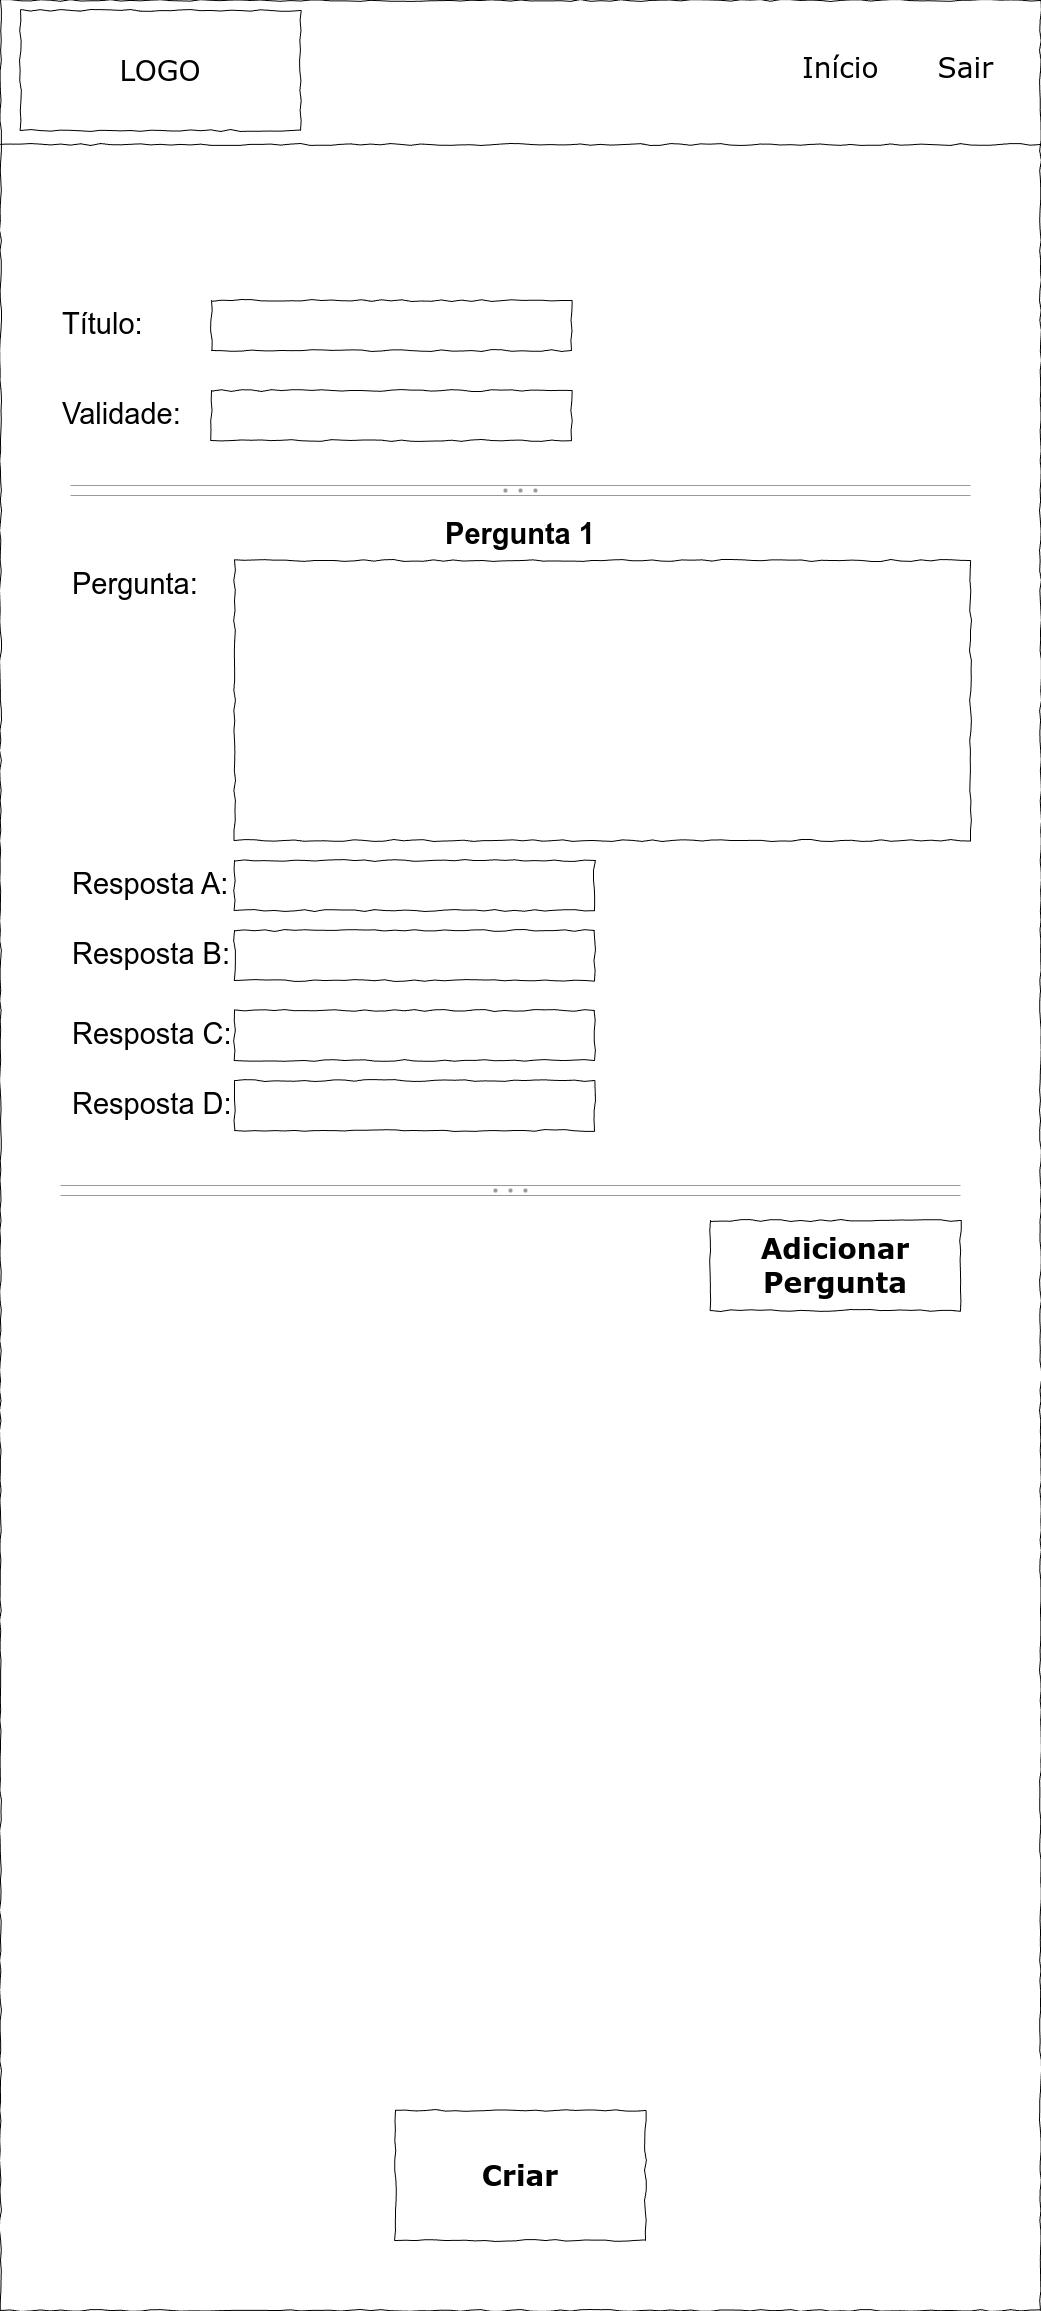
\includegraphics[width=\textwidth,height=0.9\textheight,keepaspectratio]{wireframes/questionarios.wireframes-formador-novo-questionario-mobile.drawio}
        \caption{\textit{Wireframe Mobile} - Página Novo Questionário Formador}
        \label{fig:wm-pnqf}
    \end{figure}

    \begin{figure}[H]
        \centering
        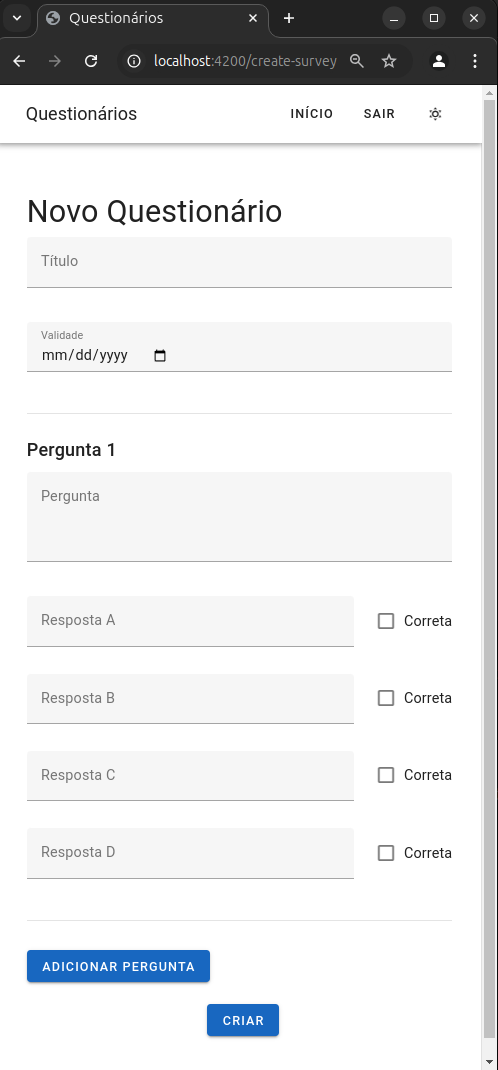
\includegraphics[width=\textwidth,height=0.9\textheight,keepaspectratio]{mockups/questionarios.wireframes-formador-novo-questionario-mobile}
        \caption{\textit{Mockup Mobile} - Página Novo Questionário Formador}
        \label{fig:mm-pnqf}
    \end{figure}

    \begin{figure}[H]
        \centering
        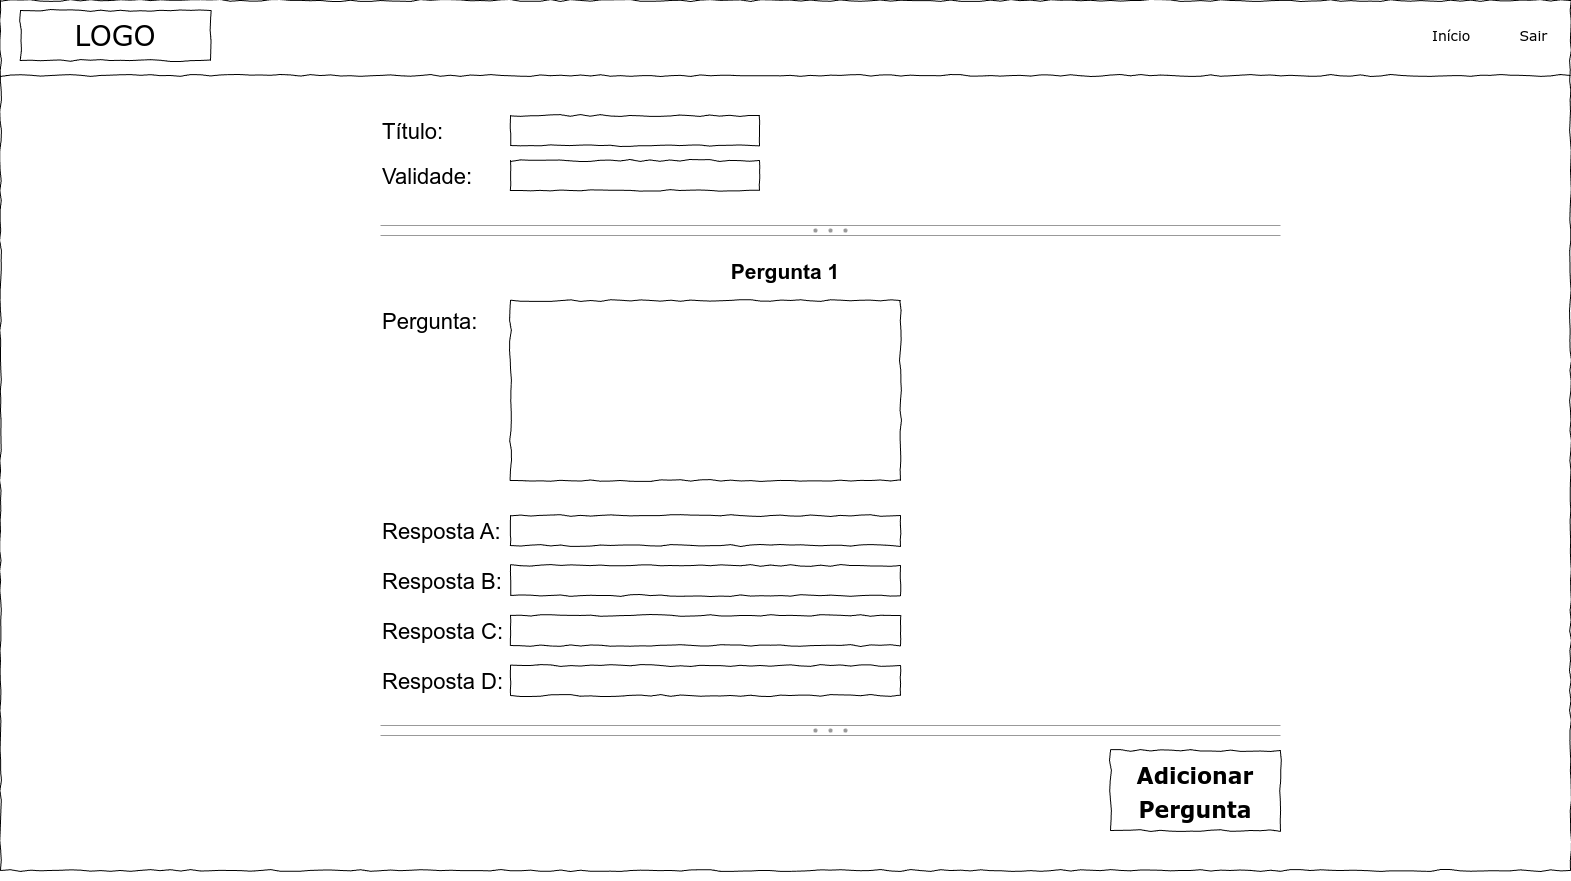
\includegraphics[width=\textwidth,height=0.9\textheight,keepaspectratio]{wireframes/questionarios.wireframes-formador-novo-questionario-desktop.drawio}
        \caption{\textit{Wireframe Desktop} - Página Novo Questionário Formador}
        \label{fig:wd-pnqf}
    \end{figure}

    \begin{figure}[H]
        \centering
        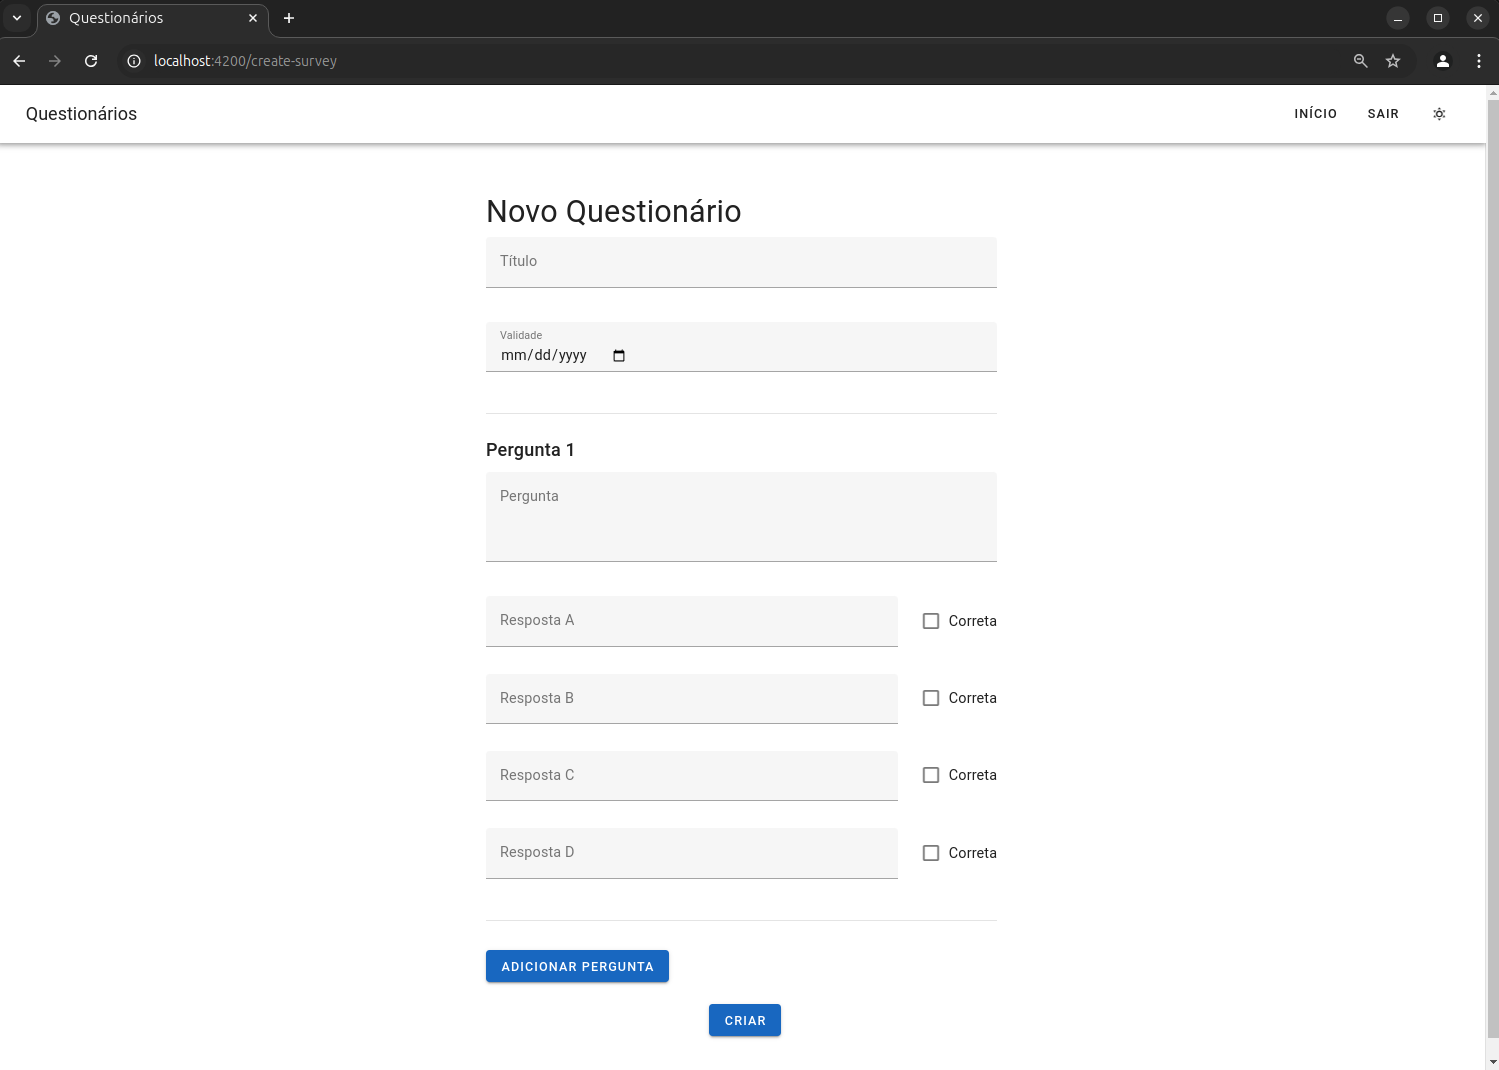
\includegraphics[width=\textwidth,height=0.9\textheight,keepaspectratio]{mockups/questionarios.wireframes-formador-novo-questionario-desktop}
        \caption{\textit{Mockup Desktop} - Página Novo Questionário Formador}
        \label{fig:md-pnqf}
    \end{figure}

    \subsection{Páginas do Estudante}\label{subsec:paginas-do-estudante}
    Para o utilizador do tipo estudante, foram consideradas duas páginas com funcionalidades específicas.

    \subsubsection{Página Inicial}
    A página inicial do utilizador do tipo estudante, apresenta uma lista de questionários por responder, permitindo aceder a cada um.

    \begin{figure}[H]
        \centering
        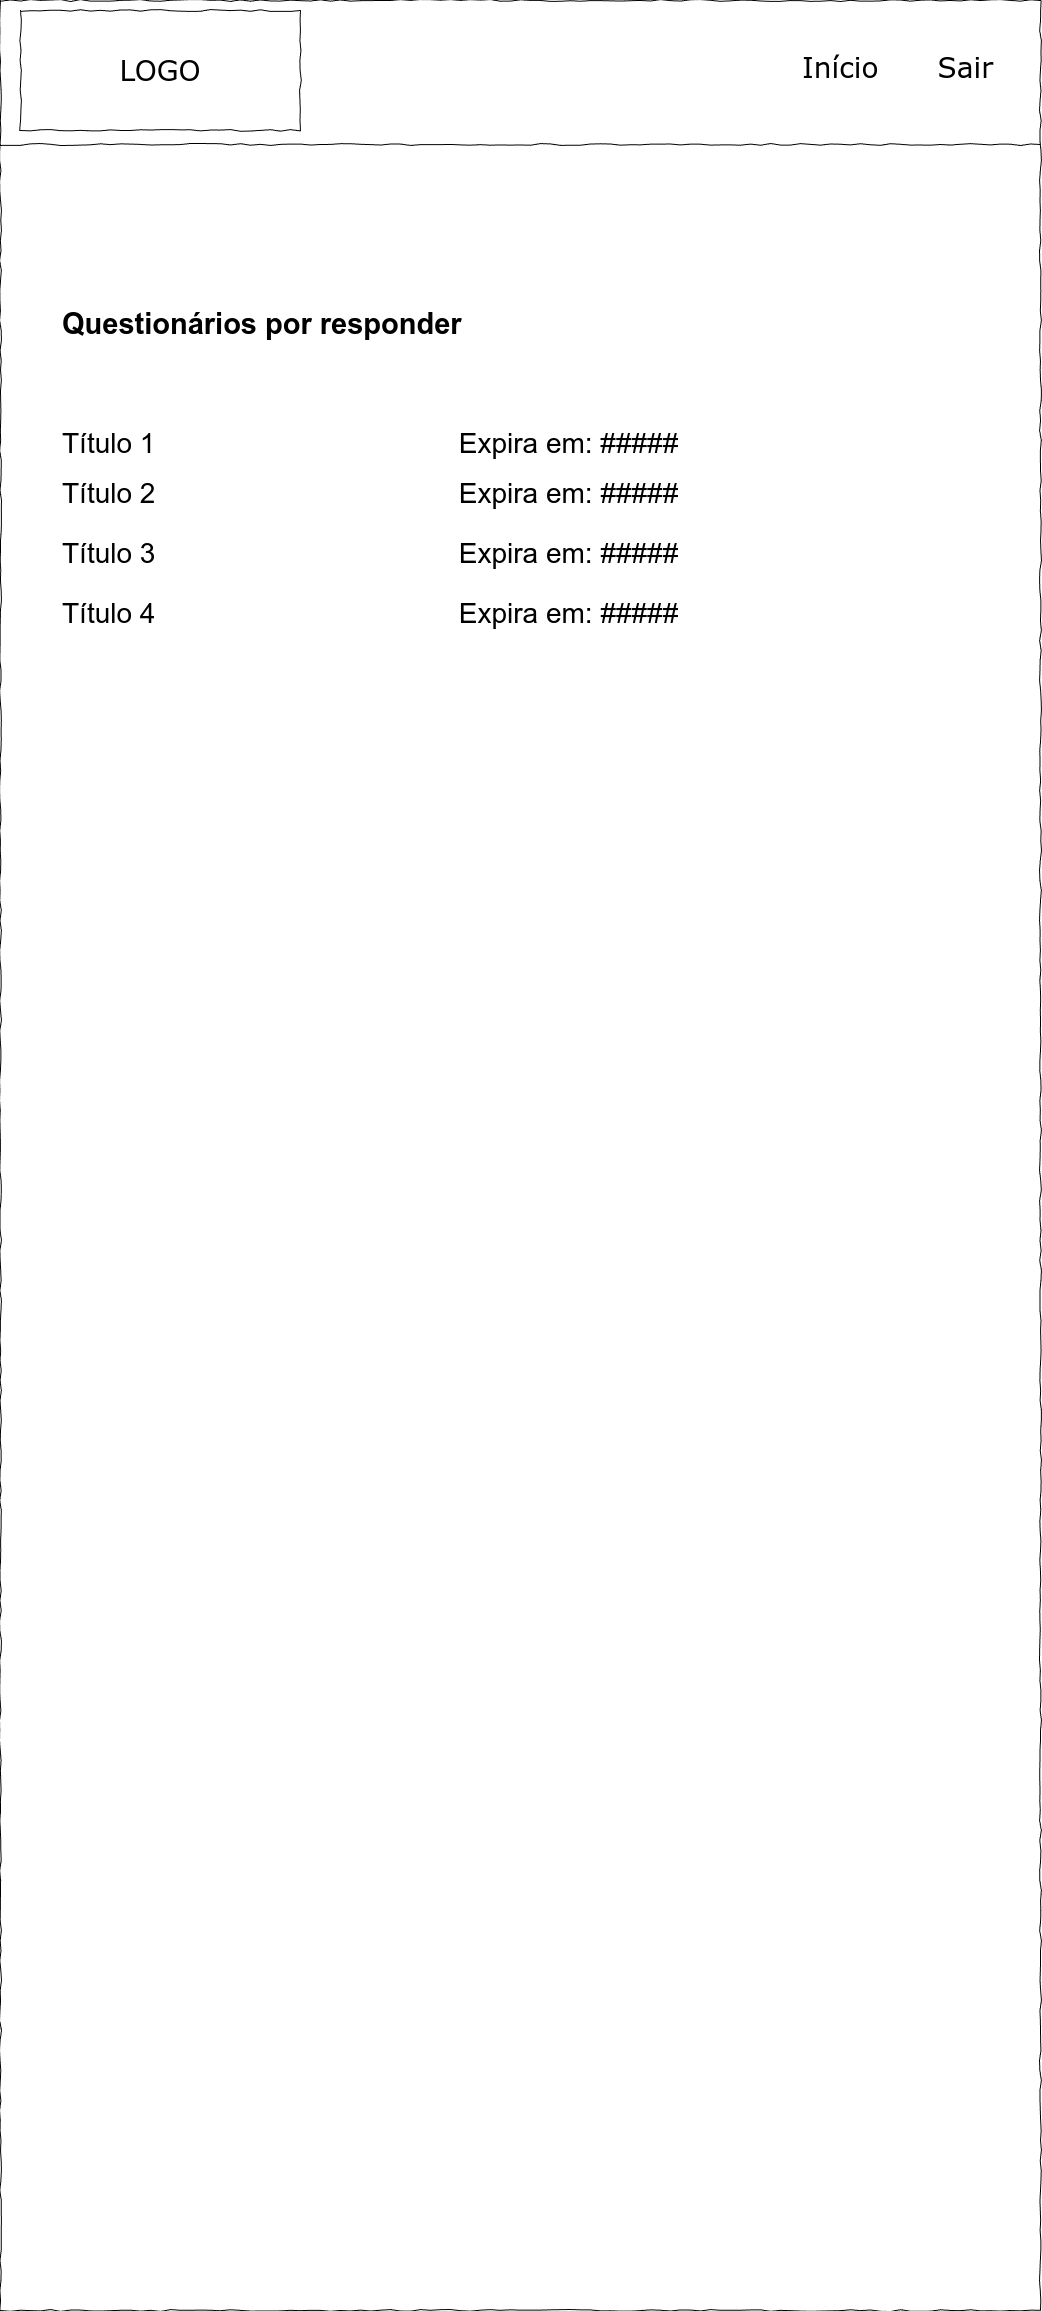
\includegraphics[width=\textwidth,height=0.9\textheight,keepaspectratio]{wireframes/questionarios.wireframes-estudante-geral-mobile.drawio}
        \caption{\textit{Wireframe Mobile} - Página Inicial Estudante}
        \label{fig:wm-pie}
    \end{figure}

    \begin{figure}[H]
        \centering
        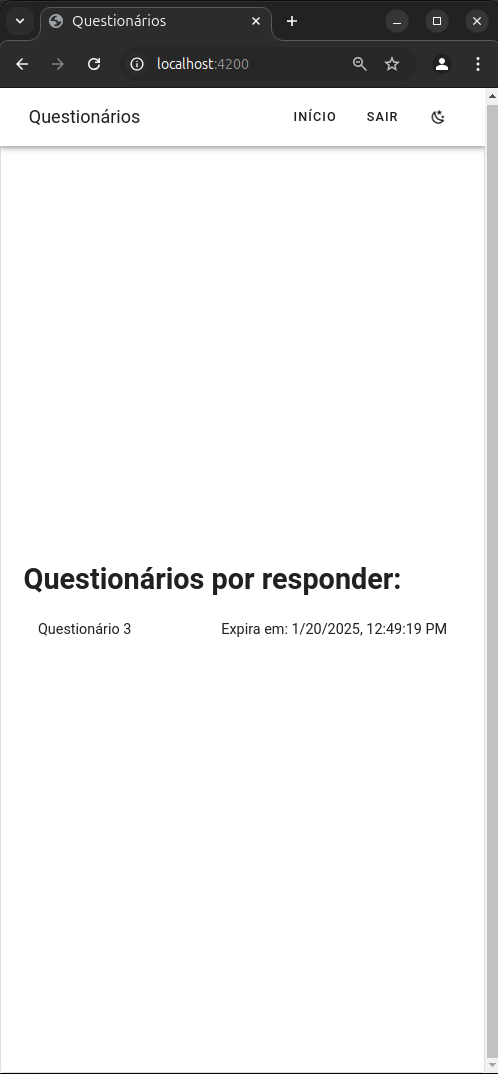
\includegraphics[width=\textwidth,height=0.9\textheight,keepaspectratio]{mockups/questionarios.wireframes-estudante-geral-mobile}
        \caption{\textit{Mockup Mobile} - Página Inicial Estudante}
        \label{fig:mm-pie}
    \end{figure}

    \begin{figure}[H]
        \centering
        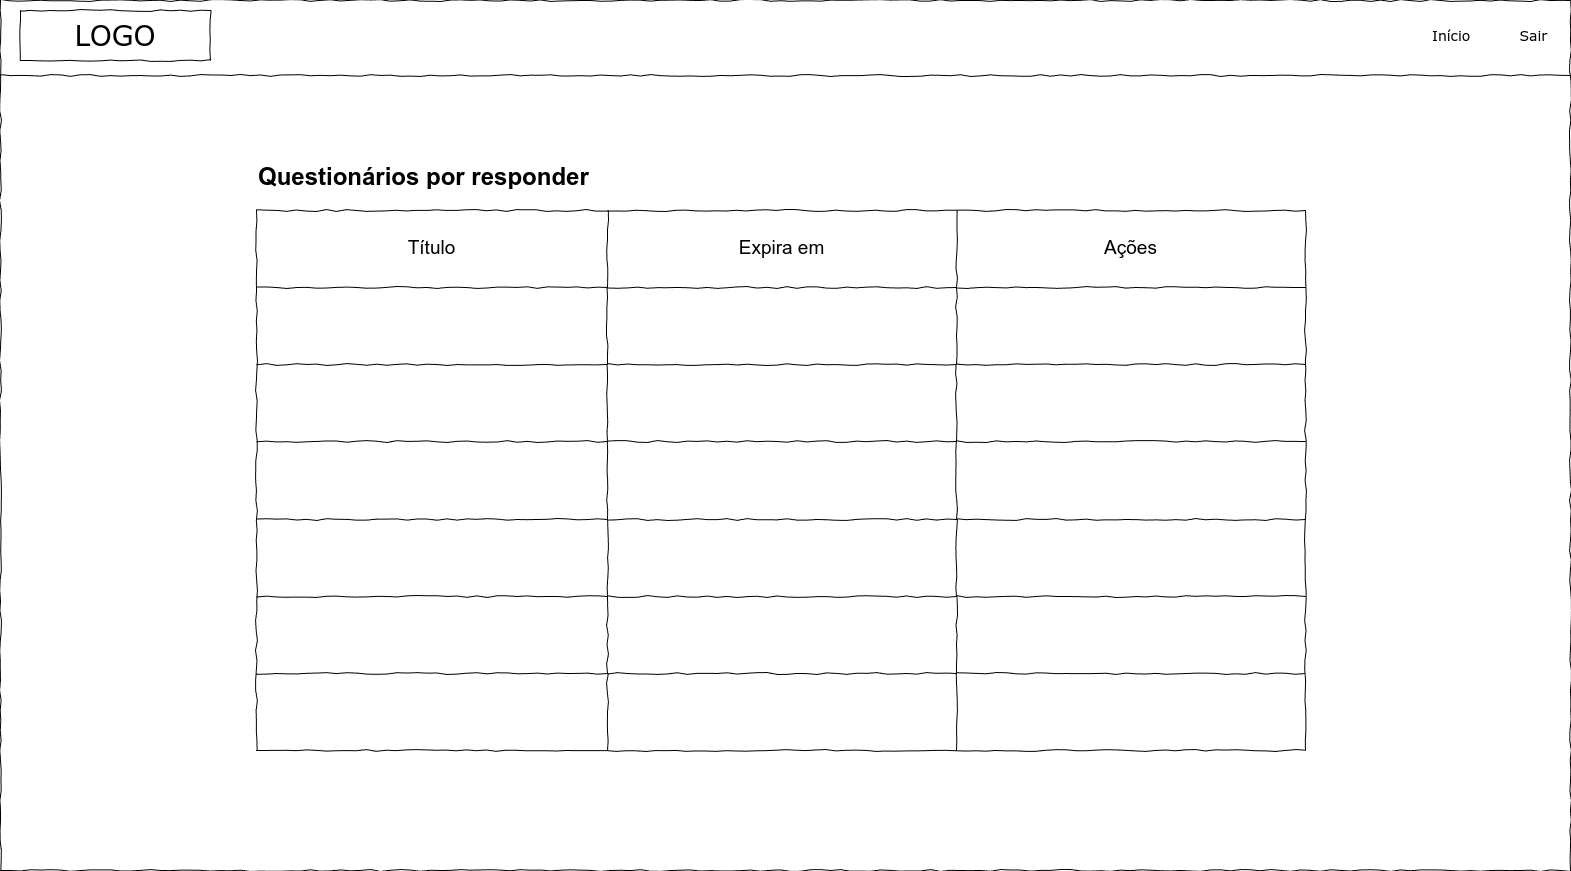
\includegraphics[width=\textwidth,height=0.9\textheight,keepaspectratio]{wireframes/questionarios.wireframes-estudante-geral-desktop.drawio}
        \caption{\textit{Wireframe Desktop} - Página Inicial Estudante}
        \label{fig:wd-pie}
    \end{figure}

    \begin{figure}[H]
        \centering
        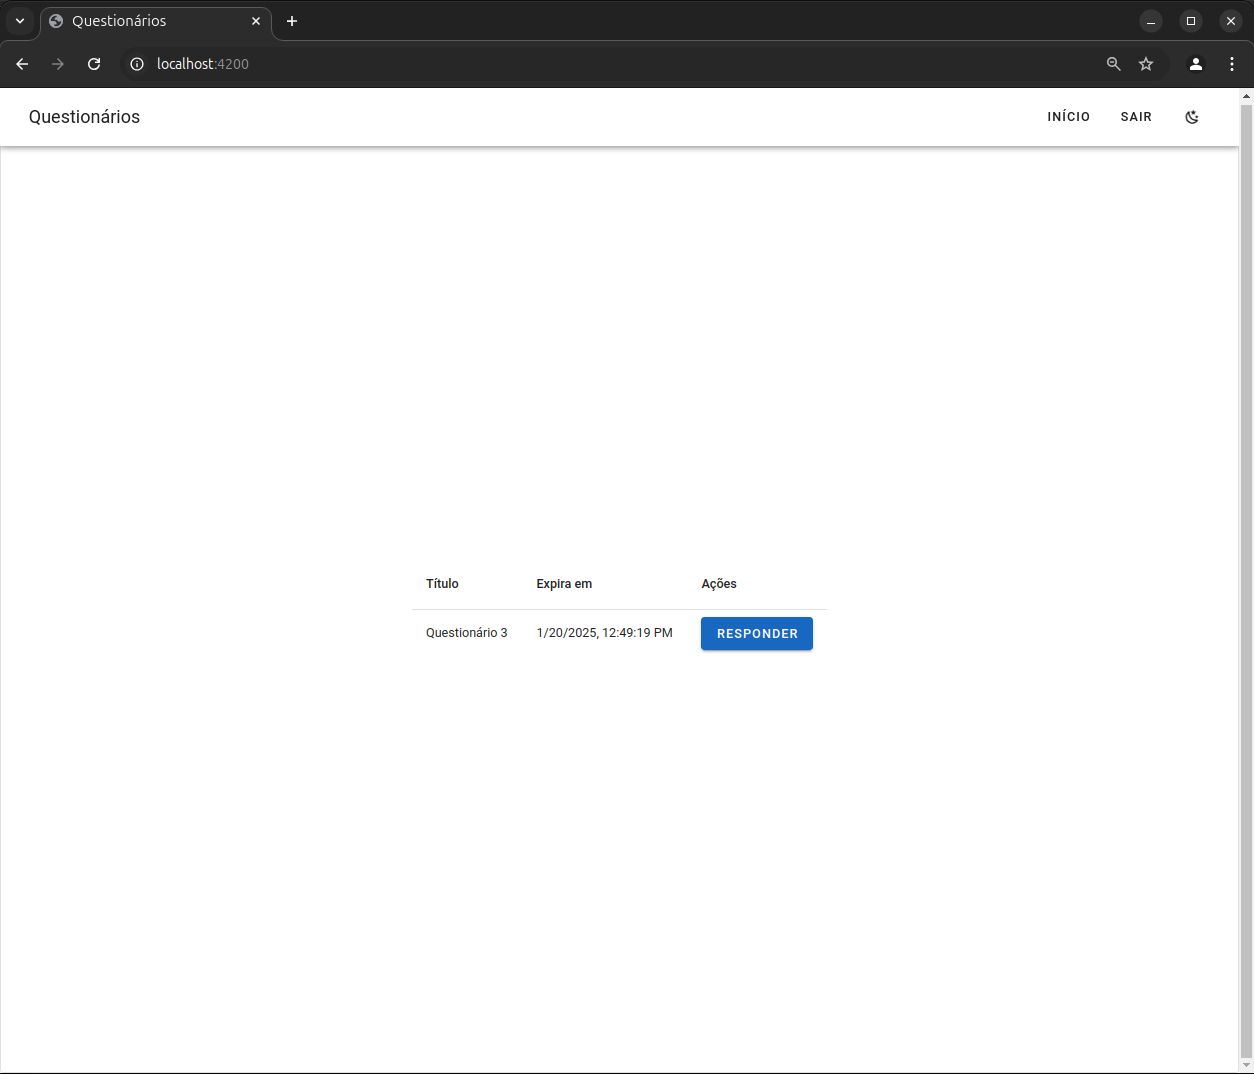
\includegraphics[width=\textwidth,height=0.9\textheight,keepaspectratio]{mockups/questionarios.wireframes-estudante-geral-desktop}
        \caption{\textit{Mockup Desktop} - Página Inicial Estudante}
        \label{fig:md-pie}
    \end{figure}

    \subsubsection{Página Questionário}
    A página questionário apresenta o título do questionário bem como as perguntas.

    \begin{figure}[H]
        \centering
        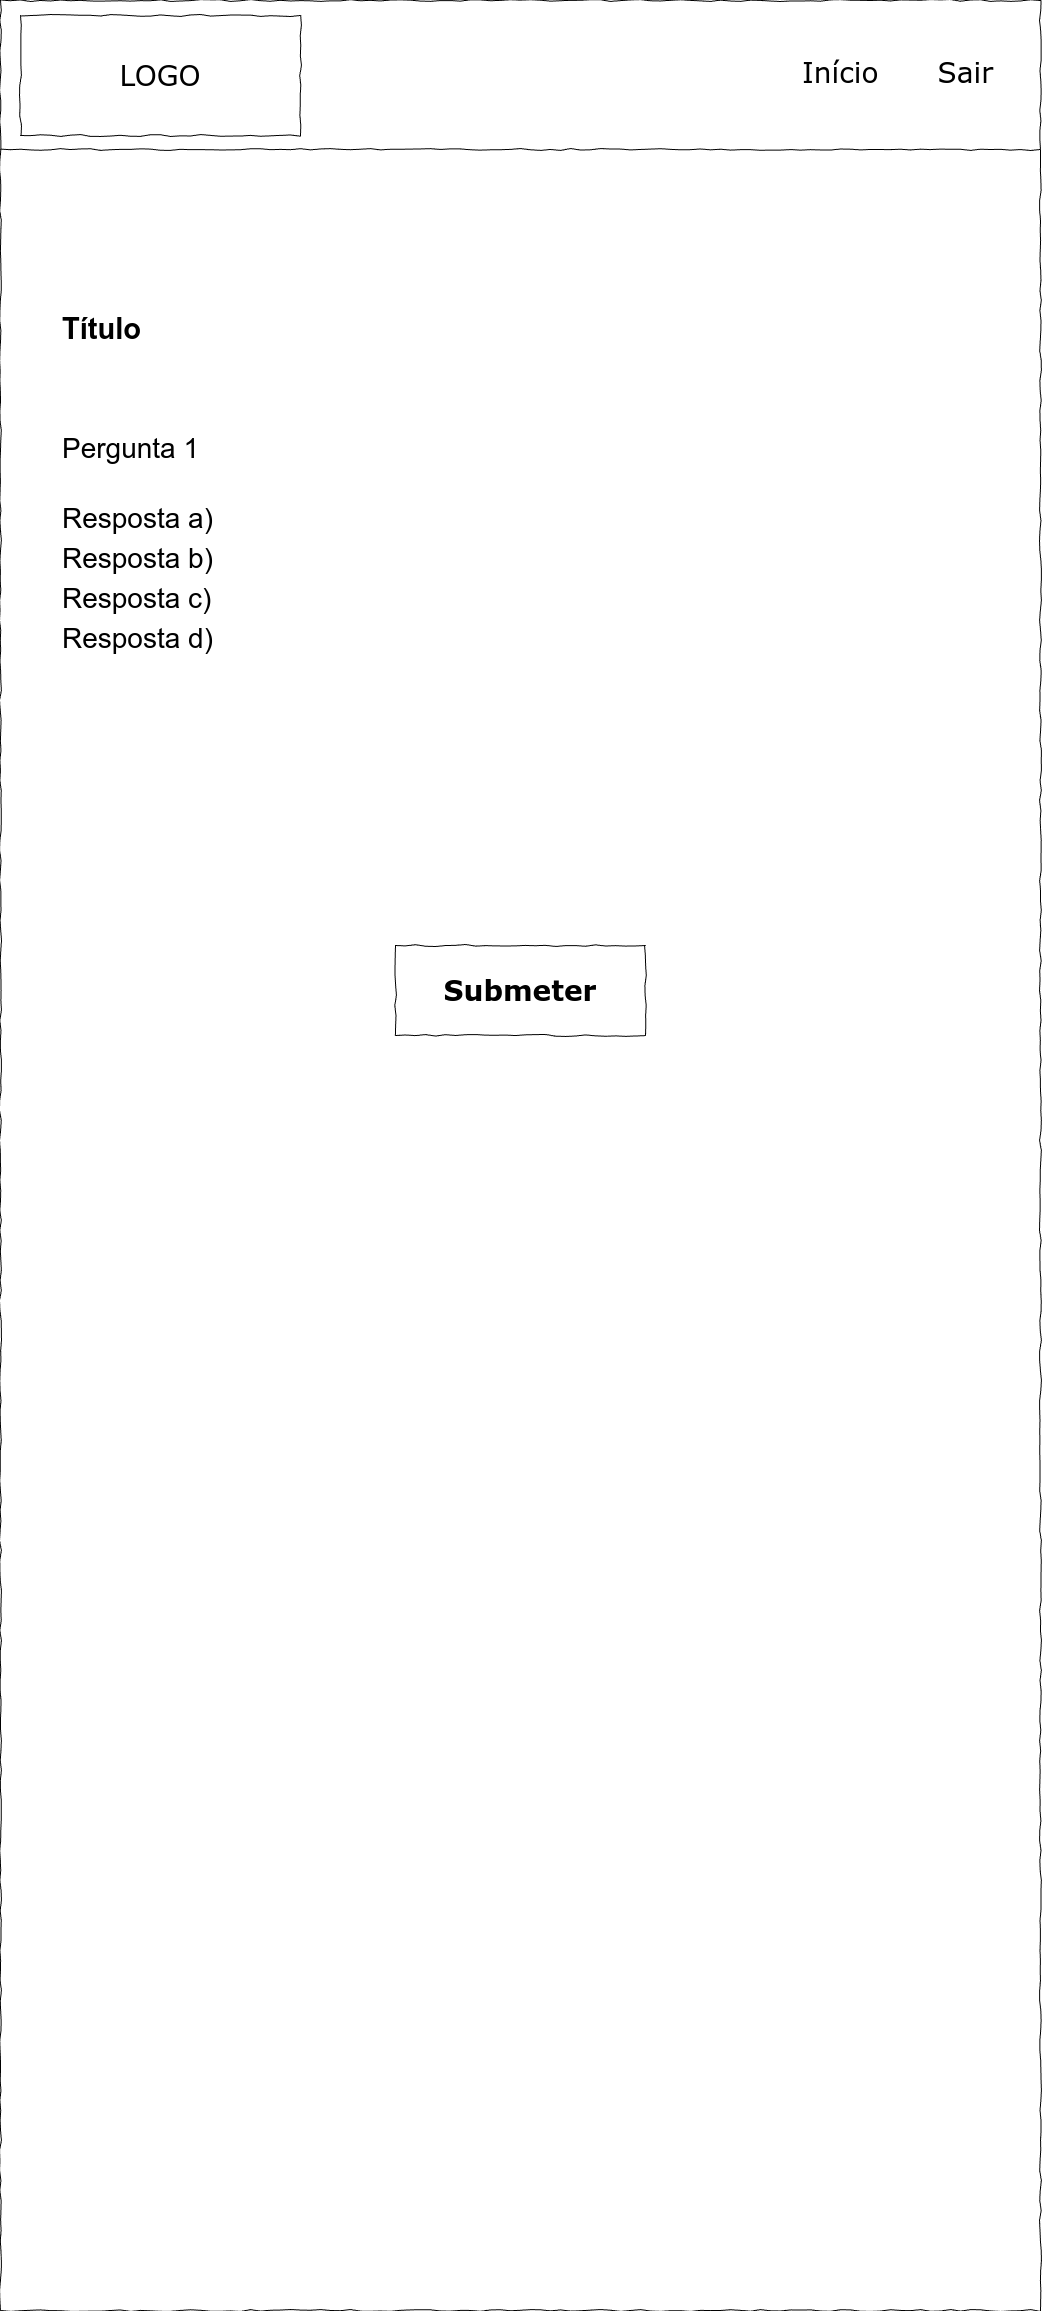
\includegraphics[width=\textwidth,height=0.9\textheight,keepaspectratio]{wireframes/questionarios.wireframes-estudante-questionario-mobile.drawio}
        \caption{\textit{Wireframe Mobile} - Página Questionário Estudante}
        \label{fig:wm-pqe}
    \end{figure}

    \begin{figure}[H]
        \centering
        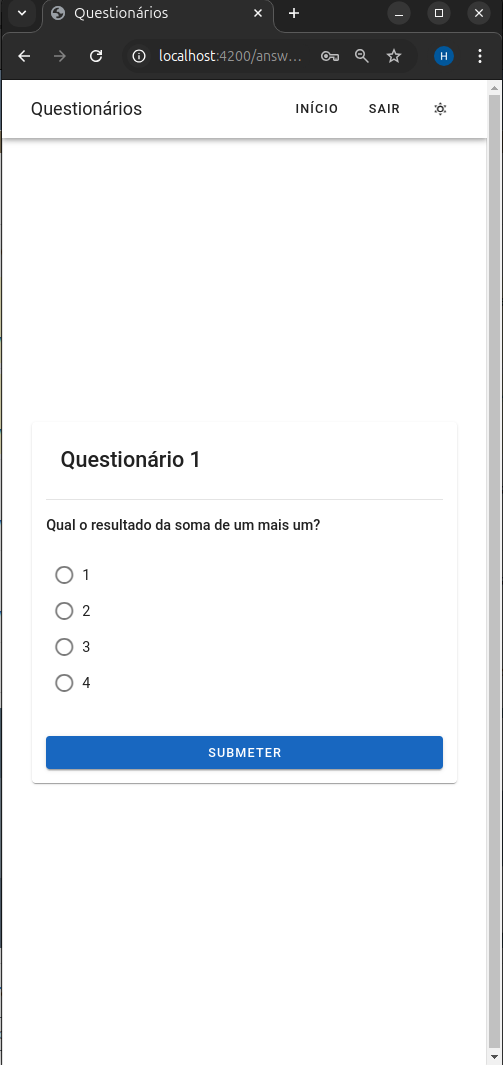
\includegraphics[width=\textwidth,height=0.9\textheight,keepaspectratio]{mockups/questionarios.wireframes-estudante-questionario-mobile}
        \caption{\textit{Mockup Mobile} - Página Questionário Estudante}
        \label{fig:mm-pqe}
    \end{figure}

    \begin{figure}[H]
        \centering
        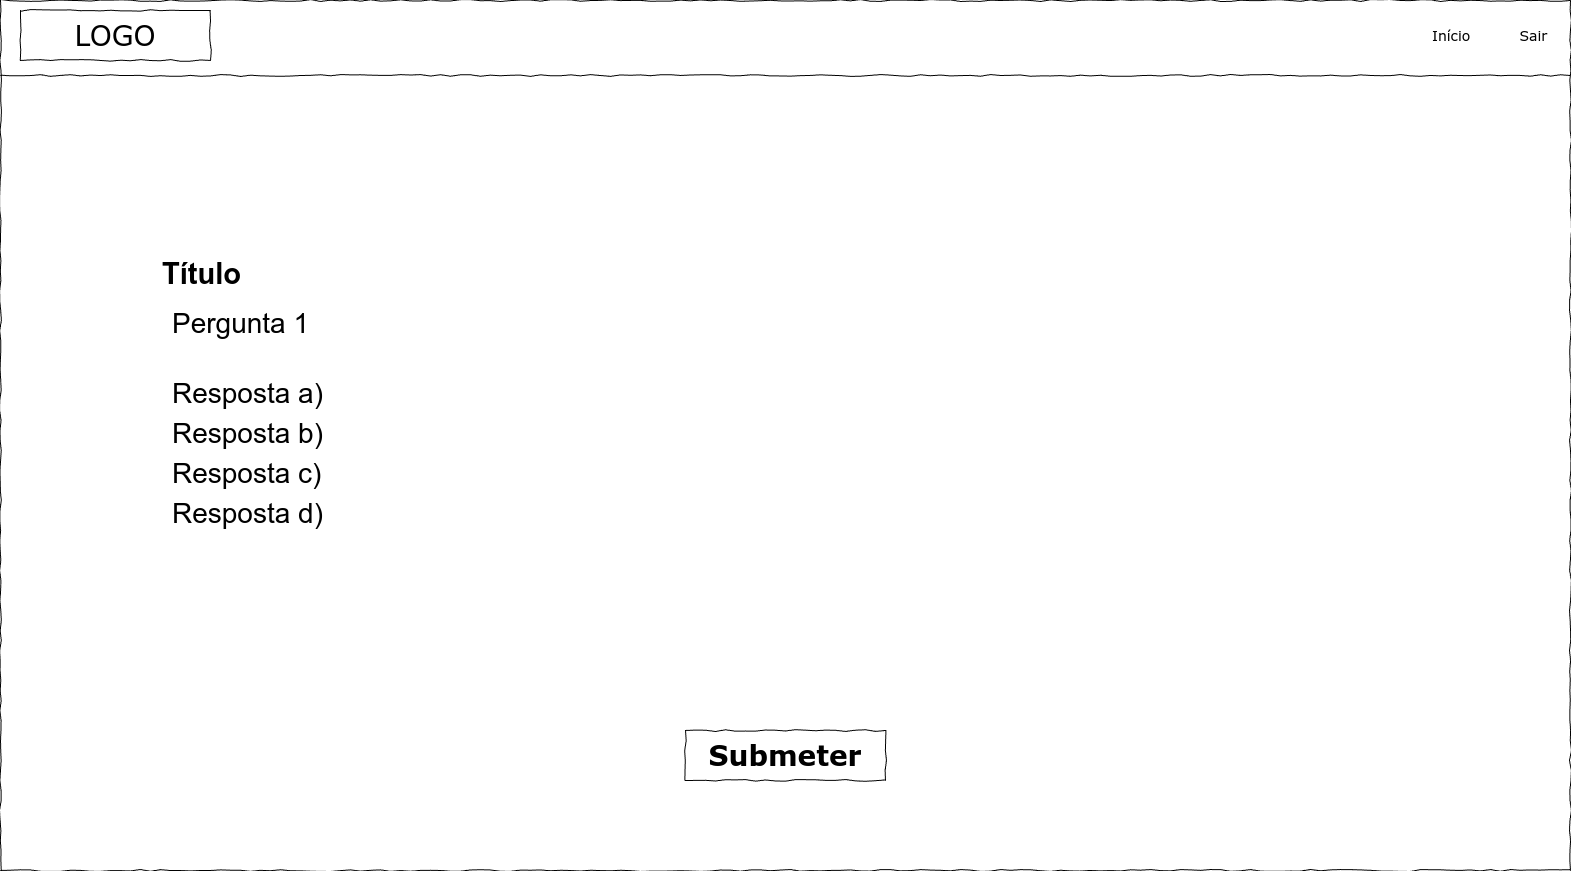
\includegraphics[width=\textwidth,height=0.9\textheight,keepaspectratio]{wireframes/questionarios.wireframes-estudante-questionario-desktop.drawio}
        \caption{\textit{Wireframe Desktop} - Página Questionário Estudante}
        \label{fig:wd-pqe}
    \end{figure}

    \begin{figure}[H]
        \centering
        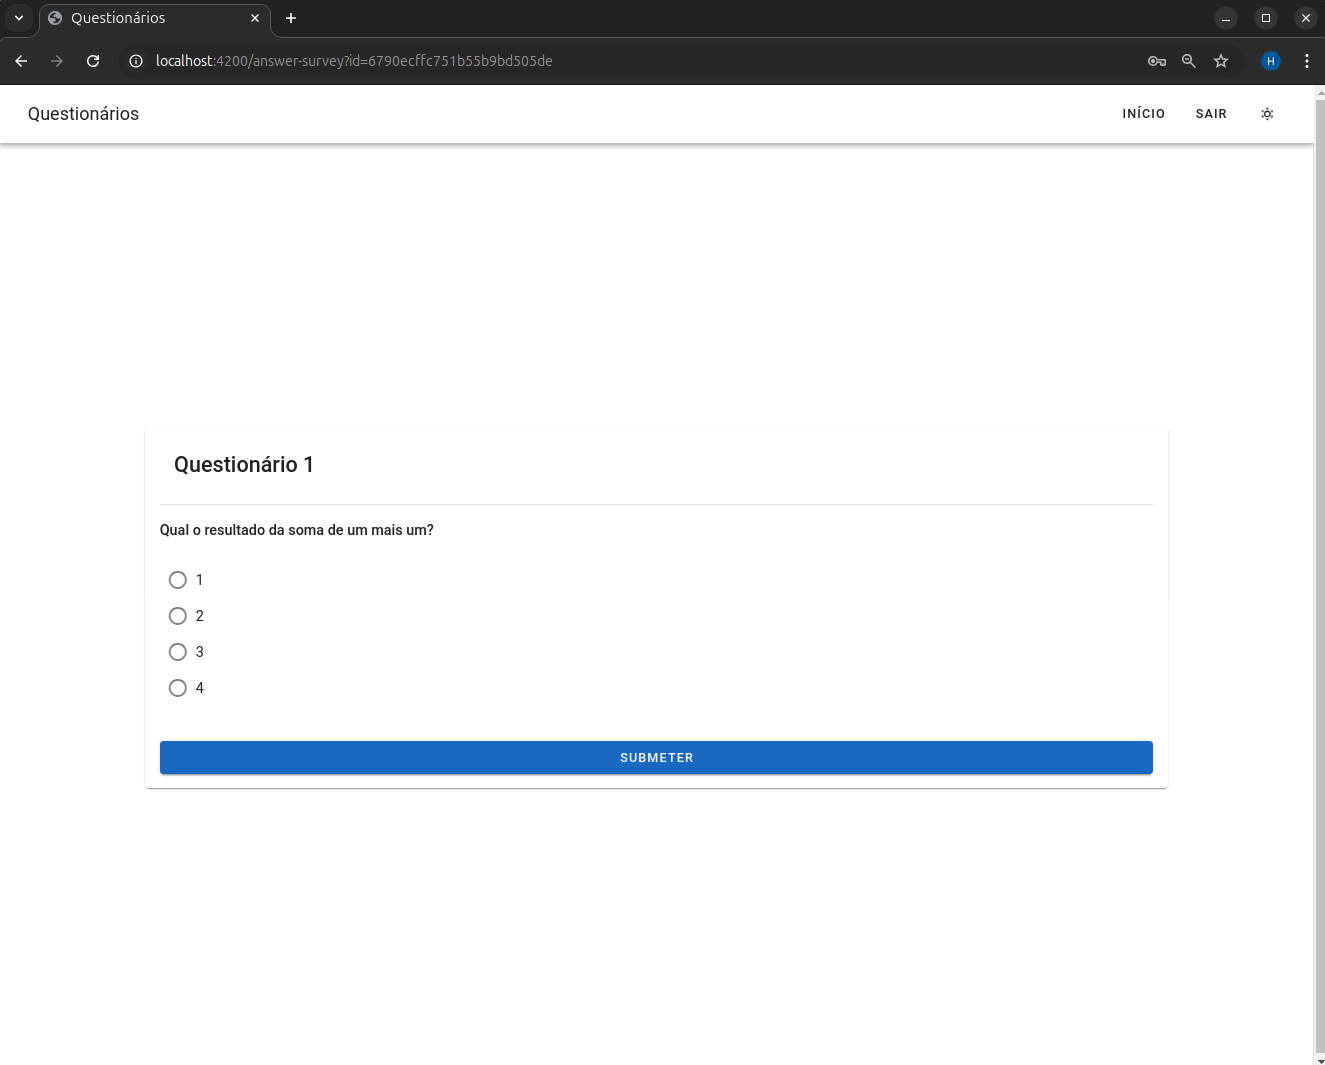
\includegraphics[width=\textwidth,height=0.9\textheight,keepaspectratio]{mockups/questionarios.wireframes-estudante-questionario-desktop}
        \caption{\textit{Mockup Desktop} - Página Questionário Estudante}
        \label{fig:md-pqe}
    \end{figure}


    \section{Técnologias Utilizadas}\label{sec:tecnologias}
    Durante o desenvolvimento da plataforma de questionários foram utilizadas diversas técnologias nos vários componentes.

    \subsection{Docker}\label{subsec:docker}
    Foi utilizado \textit{Docker} para iniciar uma base de dados NoSQL bem como uma ferramenta que permite explorar a base de dados (Mongo Express).

    \subsection{MongoDB}\label{subsec:mongodb}
    Existindo apenas duas entidades principais (\textit{user} e \textit{survey}), optou-se pela utilização de uma base de dados NoSQL, permitindo assim, que um único documento contenha tanto um questionário, como todas as respostas de estudantes, simplificando as operações no \textit{backend}.

    \subsection{Nx}\label{subsec:nx}
    O Nx permite criar \textit{monorepos} de forma simples e rápida, oferecendo utilitários para gerar automáticamente esqueletos de aplicações \textit{frontend}, \textit{backend} e bibliotecas, bem como gerar o esqueleto de \textit{unit tests} e \textit{e2e tests}.
    O Nx age também como um \textit{build system} onde podemos gerir todo o processo de desenvolvimento.

    \subsection{NestJS}\label{subsec:nestjs}
    O NestJS é uma \textit{framework} de desenvolvimento \textit{backend} para Node.js que se destaca pela sua arquitetura organizada e poderosa, baseada em TypeScript.
    Esta oferece uma estrutura robusta e escalável para criar aplicações complexas, desde APIs RESTful até microserviços.

    \subsection{Vue.js}\label{subsec:vuejs}
    Vue.js é uma \textit{framework} JavaScript de código aberto, progressiva e versátil, amplamente utilizada para construir interfaces de utilizador interativas e aplicações web.
    Esta é conhecido pela sua curva de aprendizagem suave, documentação clara e ecossistema robusto.

    \subsection{Pinia}\label{subsec:pinia}
    Pinia é uma biblioteca de gestão de estado leve e intuitiva, especialmente projetada para a \textit{framework} Vue.js.
    Esta oferece uma forma simples e eficiente de organizar e partilhar dados entre diferentes componentes de uma aplicação Vue, tornando o desenvolvimento mais escalável.

    \subsection{Vuetify}\label{subsec:vuetify}
    Vuetify é uma \textit{framework} UI (interface de utilizador) construída sobre a popular \textit{framework} JavaScript Vue.js.
    Esta oferece uma vasta coleção de componentes pré-construídos, seguindo as diretrizes do Material Design, que visam criar interfaces de utilizador modernas, responsivas e visualmente atraentes com facilidade e rapidez.


    \nocite{*}
    \newpage
    \printbibliography
\end{document}
